\begin{remark*}[Motivating picture]
Circular trigonometry reads coordinates from the unit circle
$x^2+y^2=1$. Hyperbolic trigonometry uses the same geometric idea with the
unit rectangular hyperbola
\[
  x^2-y^2=1
\]
in place of the circle. The parameter is not an angle. It is twice the signed
area of the hyperbolic sector swept from the vertex $(1,0)$ to the point on
the right branch.
\end{remark*}

\begin{center}
\makeatletter
\@ifundefined{color@atlasink}{\definecolor{atlasink}{HTML}{33312E}}{}
\@ifundefined{color@atlasgray}{\definecolor{atlasgray}{HTML}{9A958C}}{}
\@ifundefined{color@atlasblue}{\definecolor{atlasblue}{HTML}{2E6F9E}}{}
\@ifundefined{color@atlasgreen}{\definecolor{atlasgreen}{HTML}{4C8C3F}}{}
\@ifundefined{color@atlasred}{\definecolor{atlasred}{HTML}{C0473B}}{}
\@ifundefined{color@atlasgold}{\definecolor{atlasgold}{HTML}{D69A2A}}{}
\@ifundefined{atlascaption}{%
  \newcommand{\atlascaption}[3]{\shortstack{\footnotesize Figure~#1. \textbf{#2:}\\#3}}%
}{}
\@ifundefined{glowstroke}{%
  \newcommand{\glowstroke}[3]{%
    \draw[#1, line width=1.5pt, line cap=round]
      plot[domain=#2,samples=100,smooth] (\x,{#3});%
  }%
}{}
\makeatother
\tikzset{
  atlas axes/.style={atlasink, line width=0.7pt, line cap=round, ->},
  atlas curve/.style={line width=1.5pt, line cap=round, line join=round},
  dropline/.style={atlasgray, line width=0.6pt, dash pattern=on 2pt off 2pt},
  atlas dot/.style={fill=atlasink, draw=white, line width=0.4pt, circle, inner sep=0pt, minimum size=4.2pt},
}

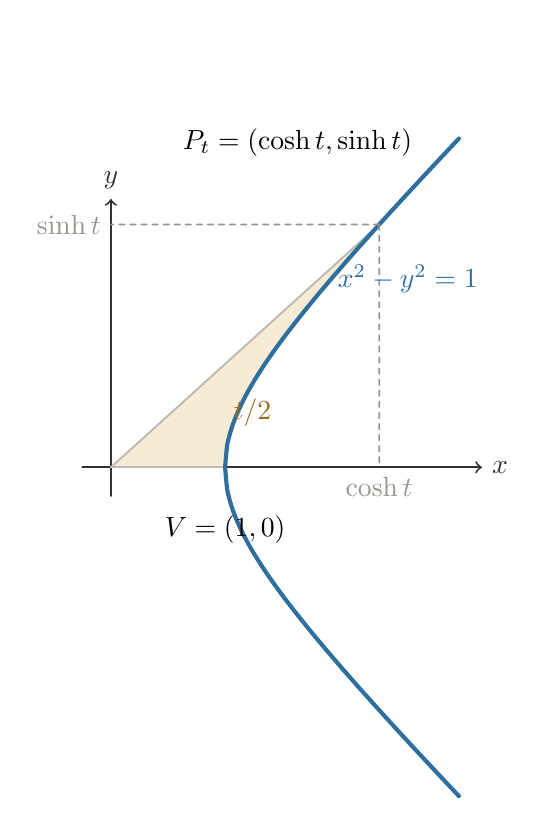
\begin{tikzpicture}[scale=1.45, line cap=round, line join=round]
  \draw[atlas axes] (-0.25,0)--(3.25,0) node[right] {$x$};
  \draw[atlas axes] (0,-0.25)--(0,2.35) node[above] {$y$};

  \fill[atlasgold!20]
    (0,0)--(1,0)
    -- plot[domain=1:2.35,samples=90,smooth] (\x,{sqrt(\x*\x-1)})
    -- cycle;
  \draw[atlasgray!65, line width=0.7pt] (0,0)--(2.35,{sqrt(2.35*2.35-1)});
  \draw[atlasgray!65, line width=0.7pt] (0,0)--(1,0);
  \draw[atlasblue, atlas curve]
    plot[domain=1:3.05,samples=120,smooth] (\x,{sqrt(\x*\x-1)});
  \draw[atlasblue, atlas curve]
    plot[domain=1:3.05,samples=120,smooth] (\x,{-sqrt(\x*\x-1)});

  \coordinate (V) at (1,0);
  \coordinate (P) at (2.35,{sqrt(2.35*2.35-1)});
  \fill[atlas dot] (V) node[below] {$V=(1,0)$};
  \fill[atlas dot] (P) node[above left] {$P_t=(\cosh t,\sinh t)$};
  \draw[dropline] (P)--(2.35,0) node[below] {$\cosh t$};
  \draw[dropline] (P)--(0,{sqrt(2.35*2.35-1)}) node[left] {$\sinh t$};
  \node[atlasgold!70!black] at (1.24,0.48) {$t/2$};
  \node[atlasblue] at (2.6,1.65) {$x^2-y^2=1$};
\end{tikzpicture}

\atlascaption{H1}{Hyperbolic sector}{The parameter $t$ is twice the shaded sector area.}
\end{center}


\begin{remark*}[Construction versus behavior]
This chapter gives the geometric construction. Continuity and differentiation
statements are recorded below as forward pointers to the later analysis
chapter on the behavior of elementary functions, where limits, continuity, and
differentiation provide the canonical proofs.
\end{remark*}
\begin{dependencies}
\begin{itemize}
  \item \hyperref[def:cartesian-product]{Cartesian Product}
  \item \hyperref[def:radian-measure]{Radian measure}
\end{itemize}
\end{dependencies}
